\documentclass[1p]{elsarticle_modified}
%\bibliographystyle{elsarticle-num}

%\usepackage[colorlinks]{hyperref}
%\usepackage{abbrmath_seonhwa} %\Abb, \Ascr, \Acal ,\Abf, \Afrak
\usepackage{amsfonts}
\usepackage{amssymb}
\usepackage{amsmath}
\usepackage{amsthm}
\usepackage{scalefnt}
\usepackage{amsbsy}
\usepackage{kotex}
\usepackage{caption}
\usepackage{subfig}
\usepackage{color}
\usepackage{graphicx}
\usepackage{xcolor} %% white, black, red, green, blue, cyan, magenta, yellow
\usepackage{float}
\usepackage{setspace}
\usepackage{hyperref}

\usepackage{tikz}
\usetikzlibrary{arrows}

\usepackage{multirow}
\usepackage{array} % fixed length table
\usepackage{hhline}

%%%%%%%%%%%%%%%%%%%%%
\makeatletter
\renewcommand*\env@matrix[1][\arraystretch]{%
	\edef\arraystretch{#1}%
	\hskip -\arraycolsep
	\let\@ifnextchar\new@ifnextchar
	\array{*\c@MaxMatrixCols c}}
\makeatother %https://tex.stackexchange.com/questions/14071/how-can-i-increase-the-line-spacing-in-a-matrix
%%%%%%%%%%%%%%%

\usepackage[normalem]{ulem}

\newcommand{\msout}[1]{\ifmmode\text{\sout{\ensuremath{#1}}}\else\sout{#1}\fi}
%SOURCE: \msout is \stkout macro in https://tex.stackexchange.com/questions/20609/strikeout-in-math-mode

\newcommand{\cancel}[1]{
	\ifmmode
	{\color{red}\msout{#1}}
	\else
	{\color{red}\sout{#1}}
	\fi
}

\newcommand{\add}[1]{
	{\color{blue}\uwave{#1}}
}

\newcommand{\replace}[2]{
	\ifmmode
	{\color{red}\msout{#1}}{\color{blue}\uwave{#2}}
	\else
	{\color{red}\sout{#1}}{\color{blue}\uwave{#2}}
	\fi
}

\newcommand{\Sol}{\mathcal{S}} %segment
\newcommand{\D}{D} %diagram
\newcommand{\A}{\mathcal{A}} %arc


%%%%%%%%%%%%%%%%%%%%%%%%%%%%%5 test

\def\sl{\operatorname{\textup{SL}}(2,\Cbb)}
\def\psl{\operatorname{\textup{PSL}}(2,\Cbb)}
\def\quan{\mkern 1mu \triangleright \mkern 1mu}

\theoremstyle{definition}
\newtheorem{thm}{Theorem}[section]
\newtheorem{prop}[thm]{Proposition}
\newtheorem{lem}[thm]{Lemma}
\newtheorem{ques}[thm]{Question}
\newtheorem{cor}[thm]{Corollary}
\newtheorem{defn}[thm]{Definition}
\newtheorem{exam}[thm]{Example}
\newtheorem{rmk}[thm]{Remark}
\newtheorem{alg}[thm]{Algorithm}

\newcommand{\I}{\sqrt{-1}}
\begin{document}

%\begin{frontmatter}
%
%\title{Boundary parabolic representations of knots up to 8 crossings}
%
%%% Group authors per affiliation:
%\author{Yunhi Cho} 
%\address{Department of Mathematics, University of Seoul, Seoul, Korea}
%\ead{yhcho@uos.ac.kr}
%
%
%\author{Seonhwa Kim} %\fnref{s_kim}}
%\address{Center for Geometry and Physics, Institute for Basic Science, Pohang, 37673, Korea}
%\ead{ryeona17@ibs.re.kr}
%
%\author{Hyuk Kim}
%\address{Department of Mathematical Sciences, Seoul National University, Seoul 08826, Korea}
%\ead{hyukkim@snu.ac.kr}
%
%\author{Seokbeom Yoon}
%\address{Department of Mathematical Sciences, Seoul National University, Seoul, 08826,  Korea}
%\ead{sbyoon15@snu.ac.kr}
%
%\begin{abstract}
%We find all boundary parabolic representation of knots up to 8 crossings.
%
%\end{abstract}
%\begin{keyword}
%    \MSC[2010] 57M25 
%\end{keyword}
%
%\end{frontmatter}

%\linenumbers
%\tableofcontents
%
\newcommand\colored[1]{\textcolor{white}{\rule[-0.35ex]{0.8em}{1.4ex}}\kern-0.8em\color{red} #1}%
%\newcommand\colored[1]{\textcolor{white}{ #1}\kern-2.17ex	\textcolor{white}{ #1}\kern-1.81ex	\textcolor{white}{ #1}\kern-2.15ex\color{red}#1	}

{\Large $\underline{12a_{0441}~(K12a_{0441})}$}

\setlength{\tabcolsep}{10pt}
\renewcommand{\arraystretch}{1.6}
\vspace{1cm}\begin{tabular}{m{100pt}>{\centering\arraybackslash}m{274pt}}
\multirow{5}{120pt}{
	\centering
	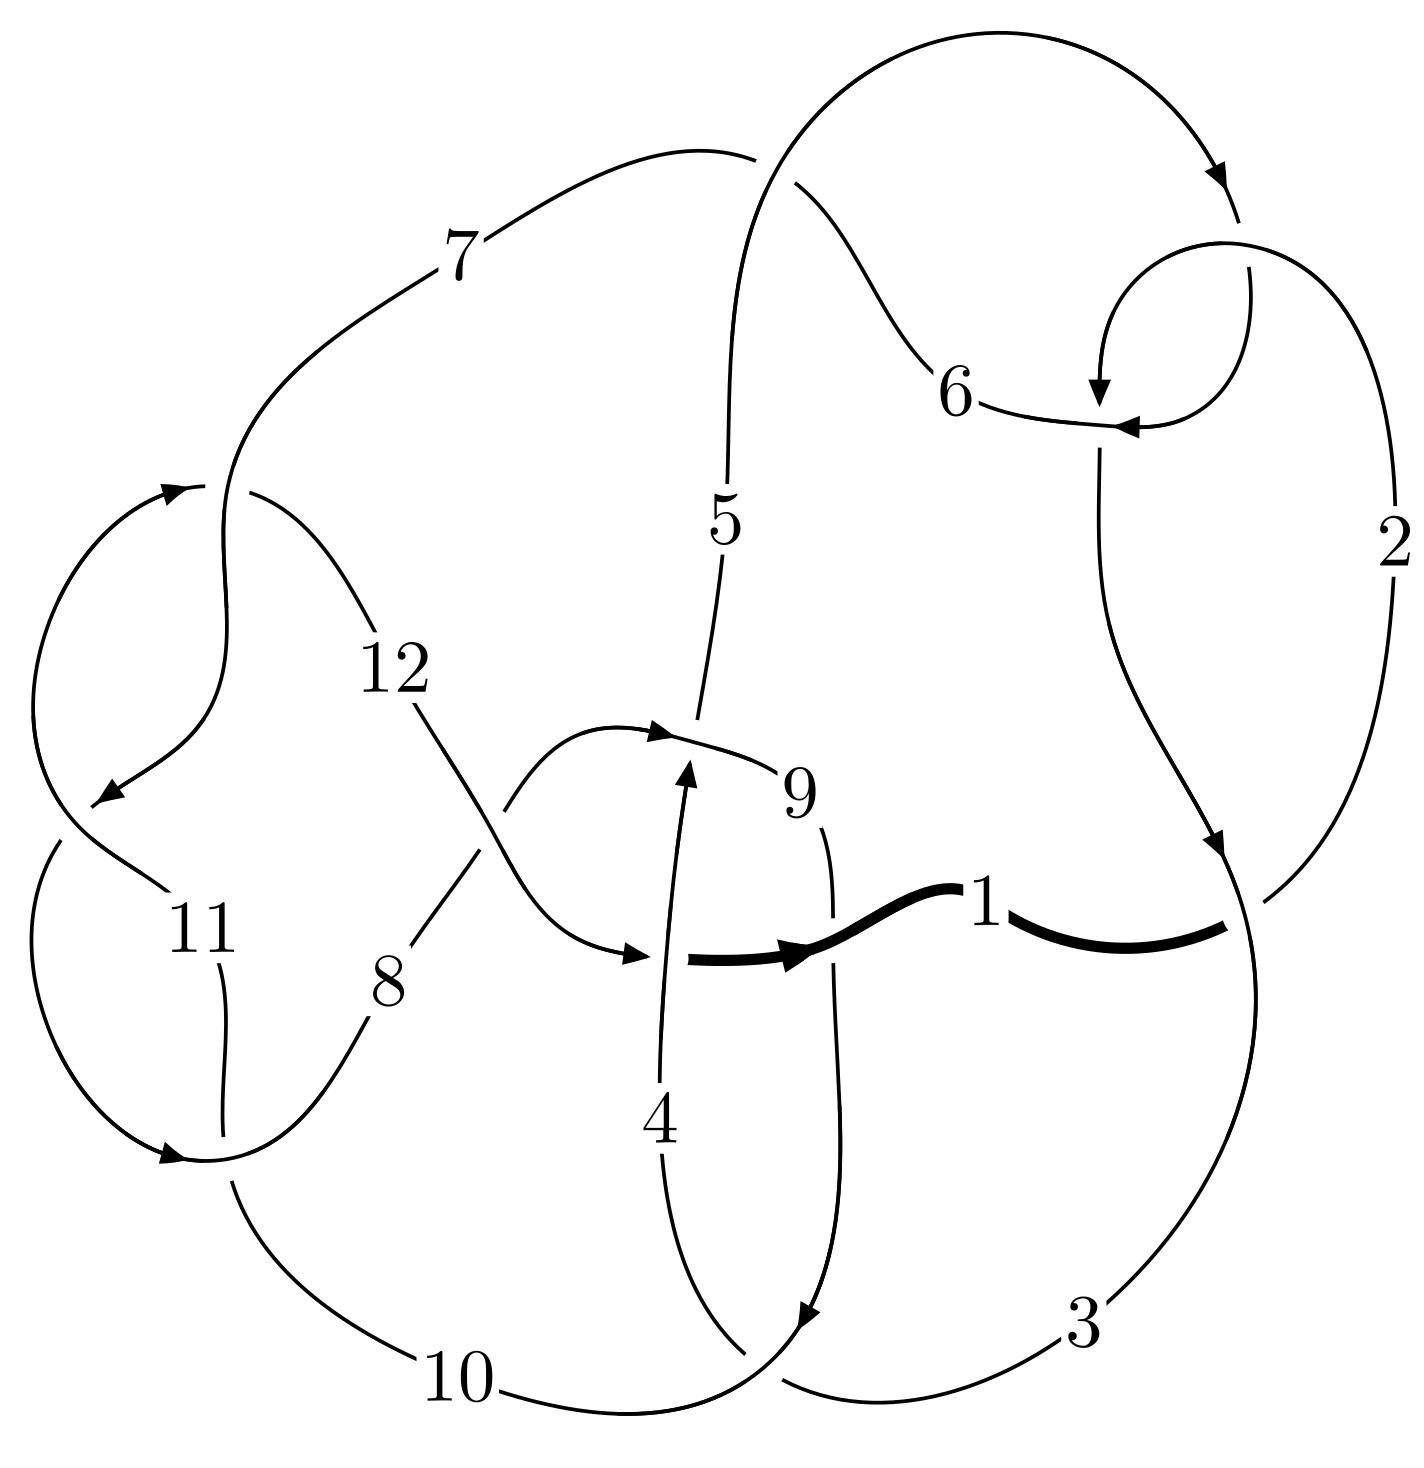
\includegraphics[width=112pt]{../../../GIT/diagram.site/Diagrams/png/1242_12a_0441.png}\\
\ \ \ A knot diagram\footnotemark}&
\allowdisplaybreaks
\textbf{Linearized knot diagam} \\
\cline{2-2}
 &
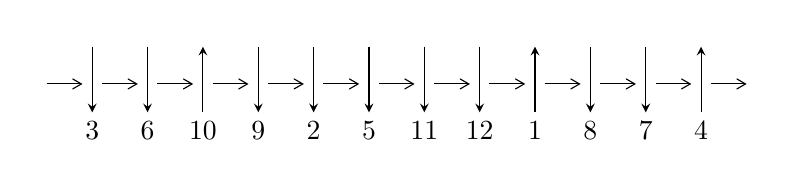
\begin{tikzpicture}[x=20pt, y=17pt]
	% nodes
	\node (C0) at (0, 0) {};
	\node (C1) at (1, 0) {};
	\node (C1U) at (1, +1) {};
	\node (C1D) at (1, -1) {3};

	\node (C2) at (2, 0) {};
	\node (C2U) at (2, +1) {};
	\node (C2D) at (2, -1) {6};

	\node (C3) at (3, 0) {};
	\node (C3U) at (3, +1) {};
	\node (C3D) at (3, -1) {10};

	\node (C4) at (4, 0) {};
	\node (C4U) at (4, +1) {};
	\node (C4D) at (4, -1) {9};

	\node (C5) at (5, 0) {};
	\node (C5U) at (5, +1) {};
	\node (C5D) at (5, -1) {2};

	\node (C6) at (6, 0) {};
	\node (C6U) at (6, +1) {};
	\node (C6D) at (6, -1) {5};

	\node (C7) at (7, 0) {};
	\node (C7U) at (7, +1) {};
	\node (C7D) at (7, -1) {11};

	\node (C8) at (8, 0) {};
	\node (C8U) at (8, +1) {};
	\node (C8D) at (8, -1) {12};

	\node (C9) at (9, 0) {};
	\node (C9U) at (9, +1) {};
	\node (C9D) at (9, -1) {1};

	\node (C10) at (10, 0) {};
	\node (C10U) at (10, +1) {};
	\node (C10D) at (10, -1) {8};

	\node (C11) at (11, 0) {};
	\node (C11U) at (11, +1) {};
	\node (C11D) at (11, -1) {7};

	\node (C12) at (12, 0) {};
	\node (C12U) at (12, +1) {};
	\node (C12D) at (12, -1) {4};
	\node (C13) at (13, 0) {};

	% arrows
	\draw[->,>={angle 60}]
	(C0) edge (C1) (C1) edge (C2) (C2) edge (C3) (C3) edge (C4) (C4) edge (C5) (C5) edge (C6) (C6) edge (C7) (C7) edge (C8) (C8) edge (C9) (C9) edge (C10) (C10) edge (C11) (C11) edge (C12) (C12) edge (C13) ;	\draw[->,>=stealth]
	(C1U) edge (C1D) (C2U) edge (C2D) (C3D) edge (C3U) (C4U) edge (C4D) (C5U) edge (C5D) (C6U) edge (C6D) (C7U) edge (C7D) (C8U) edge (C8D) (C9D) edge (C9U) (C10U) edge (C10D) (C11U) edge (C11D) (C12D) edge (C12U) ;
	\end{tikzpicture} \\
\hhline{~~} \\& 
\textbf{Solving Sequence} \\ \cline{2-2} 
 &
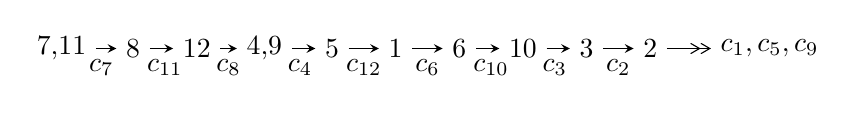
\begin{tikzpicture}[x=23pt, y=7pt]
	% node
	\node (A0) at (-1/8, 0) {7,11};
	\node (A1) at (1, 0) {8};
	\node (A2) at (2, 0) {12};
	\node (A3) at (49/16, 0) {4,9};
	\node (A4) at (33/8, 0) {5};
	\node (A5) at (41/8, 0) {1};
	\node (A6) at (49/8, 0) {6};
	\node (A7) at (57/8, 0) {10};
	\node (A8) at (65/8, 0) {3};
	\node (A9) at (73/8, 0) {2};
	\node (C1) at (1/2, -1) {$c_{7}$};
	\node (C2) at (3/2, -1) {$c_{11}$};
	\node (C3) at (5/2, -1) {$c_{8}$};
	\node (C4) at (29/8, -1) {$c_{4}$};
	\node (C5) at (37/8, -1) {$c_{12}$};
	\node (C6) at (45/8, -1) {$c_{6}$};
	\node (C7) at (53/8, -1) {$c_{10}$};
	\node (C8) at (61/8, -1) {$c_{3}$};
	\node (C9) at (69/8, -1) {$c_{2}$};
	\node (A10) at (11, 0) {$c_{1},c_{5},c_{9}$};

	% edge
	\draw[->,>=stealth]	
	(A0) edge (A1) (A1) edge (A2) (A2) edge (A3) (A3) edge (A4) (A4) edge (A5) (A5) edge (A6) (A6) edge (A7) (A7) edge (A8) (A8) edge (A9) ;
	\draw[->>,>={angle 60}]	
	(A9) edge (A10);
\end{tikzpicture} \\ 

\end{tabular} \\

\footnotetext{
The image of knot diagram is generated by the software ``\textbf{Draw programme}" developed by Andrew Bartholomew(\url{http://www.layer8.co.uk/maths/draw/index.htm\#Running-draw}), where we modified some parts for our purpose(\url{https://github.com/CATsTAILs/LinksPainter}).
}\phantom \\ \newline 
\centering \textbf{Ideals for irreducible components\footnotemark of $X_{\text{par}}$} 
 
\begin{align*}
I^u_{1}&=\langle 
3.27711\times10^{102} u^{101}+1.55836\times10^{103} u^{100}+\cdots+2.62772\times10^{103} b-1.25743\times10^{103},\\
\phantom{I^u_{1}}&\phantom{= \langle  }3.78313\times10^{102} u^{101}-5.58370\times10^{102} u^{100}+\cdots+2.62772\times10^{103} a-4.51200\times10^{103},\;u^{102}+2 u^{101}+\cdots+4 u-1\rangle \\
I^u_{2}&=\langle 
b- u+1,\;u^2+a+1,\;u^3- u^2+2 u-1\rangle \\
\\
\end{align*}
\raggedright * 2 irreducible components of $\dim_{\mathbb{C}}=0$, with total 105 representations.\\
\footnotetext{All coefficients of polynomials are rational numbers. But the coefficients are sometimes approximated in decimal forms when there is not enough margin.}
\newpage
\renewcommand{\arraystretch}{1}
\centering \section*{I. $I^u_{1}= \langle 3.28\times10^{102} u^{101}+1.56\times10^{103} u^{100}+\cdots+2.63\times10^{103} b-1.26\times10^{103},\;3.78\times10^{102} u^{101}-5.58\times10^{102} u^{100}+\cdots+2.63\times10^{103} a-4.51\times10^{103},\;u^{102}+2 u^{101}+\cdots+4 u-1 \rangle$}
\flushleft \textbf{(i) Arc colorings}\\
\begin{tabular}{m{7pt} m{180pt} m{7pt} m{180pt} }
\flushright $a_{7}=$&$\begin{pmatrix}1\\0\end{pmatrix}$ \\
\flushright $a_{11}=$&$\begin{pmatrix}0\\u\end{pmatrix}$ \\
\flushright $a_{8}=$&$\begin{pmatrix}1\\u^2\end{pmatrix}$ \\
\flushright $a_{12}=$&$\begin{pmatrix}- u\\u\end{pmatrix}$ \\
\flushright $a_{4}=$&$\begin{pmatrix}-0.143970 u^{101}+0.212492 u^{100}+\cdots-15.9951 u+1.71708\\-0.124713 u^{101}-0.593046 u^{100}+\cdots-1.79673 u+0.478524\end{pmatrix}$ \\
\flushright $a_{9}=$&$\begin{pmatrix}- u^4- u^2+1\\u^4+2 u^2\end{pmatrix}$ \\
\flushright $a_{5}=$&$\begin{pmatrix}-0.0438647 u^{101}+0.121507 u^{100}+\cdots-17.6760 u+1.94288\\0.0129440 u^{101}+0.0941687 u^{100}+\cdots-2.42475 u+0.661696\end{pmatrix}$ \\
\flushright $a_{1}=$&$\begin{pmatrix}0.340303 u^{101}+0.920651 u^{100}+\cdots+4.12833 u-3.41343\\0.0802727 u^{101}-0.159772 u^{100}+\cdots+5.51631 u-0.420576\end{pmatrix}$ \\
\flushright $a_{6}=$&$\begin{pmatrix}0.280386 u^{101}+0.439282 u^{100}+\cdots+4.90809 u-0.660980\\0.0907918 u^{101}+0.172191 u^{100}+\cdots+2.45351 u-0.598287\end{pmatrix}$ \\
\flushright $a_{10}=$&$\begin{pmatrix}u\\u^3+u\end{pmatrix}$ \\
\flushright $a_{3}=$&$\begin{pmatrix}-0.0822981 u^{101}+0.0664369 u^{100}+\cdots-18.3878 u+2.28500\\0.0138280 u^{101}+0.101020 u^{100}+\cdots-3.05023 u+0.777047\end{pmatrix}$ \\
\flushright $a_{2}=$&$\begin{pmatrix}-0.0489390 u^{101}-0.0545099 u^{100}+\cdots-0.777862 u-1.55095\\0.00990874 u^{101}-0.00655573 u^{100}+\cdots+2.52993 u+0.271094\end{pmatrix}$\\&\end{tabular}
\flushleft \textbf{(ii) Obstruction class $= -1$}\\~\\
\flushleft \textbf{(iii) Cusp Shapes $= -0.789125 u^{101}-1.26697 u^{100}+\cdots-29.4788 u-4.11553$}\\~\\
\newpage\renewcommand{\arraystretch}{1}
\flushleft \textbf{(iv) u-Polynomials at the component}\newline \\
\begin{tabular}{m{50pt}|m{274pt}}
Crossings & \hspace{64pt}u-Polynomials at each crossing \\
\hline $$\begin{aligned}c_{1},c_{6}\end{aligned}$$&$\begin{aligned}
&u^{102}+32 u^{101}+\cdots-3 u+1
\end{aligned}$\\
\hline $$\begin{aligned}c_{2},c_{5}\end{aligned}$$&$\begin{aligned}
&u^{102}+4 u^{101}+\cdots+11 u+1
\end{aligned}$\\
\hline $$\begin{aligned}c_{3}\end{aligned}$$&$\begin{aligned}
&u^{102}+2 u^{101}+\cdots+5470 u-5977
\end{aligned}$\\
\hline $$\begin{aligned}c_{4}\end{aligned}$$&$\begin{aligned}
&u^{102}+4 u^{101}+\cdots-19212 u+1231
\end{aligned}$\\
\hline $$\begin{aligned}c_{7},c_{10},c_{11}\end{aligned}$$&$\begin{aligned}
&u^{102}-2 u^{101}+\cdots-4 u-1
\end{aligned}$\\
\hline $$\begin{aligned}c_{8}\end{aligned}$$&$\begin{aligned}
&u^{102}+2 u^{101}+\cdots-18596 u-1873
\end{aligned}$\\
\hline $$\begin{aligned}c_{9}\end{aligned}$$&$\begin{aligned}
&u^{102}-7 u^{101}+\cdots-12 u+8
\end{aligned}$\\
\hline $$\begin{aligned}c_{12}\end{aligned}$$&$\begin{aligned}
&u^{102}+10 u^{101}+\cdots+u-1
\end{aligned}$\\
\hline
\end{tabular}\\~\\
\newpage\renewcommand{\arraystretch}{1}
\flushleft \textbf{(v) Riley Polynomials at the component}\newline \\
\begin{tabular}{m{50pt}|m{274pt}}
Crossings & \hspace{64pt}Riley Polynomials at each crossing \\
\hline $$\begin{aligned}c_{1},c_{6}\end{aligned}$$&$\begin{aligned}
&y^{102}+80 y^{101}+\cdots+523 y+1
\end{aligned}$\\
\hline $$\begin{aligned}c_{2},c_{5}\end{aligned}$$&$\begin{aligned}
&y^{102}-32 y^{101}+\cdots+3 y+1
\end{aligned}$\\
\hline $$\begin{aligned}c_{3}\end{aligned}$$&$\begin{aligned}
&y^{102}-126 y^{101}+\cdots-2034750148 y+35724529
\end{aligned}$\\
\hline $$\begin{aligned}c_{4}\end{aligned}$$&$\begin{aligned}
&y^{102}-98 y^{101}+\cdots-154232356 y+1515361
\end{aligned}$\\
\hline $$\begin{aligned}c_{7},c_{10},c_{11}\end{aligned}$$&$\begin{aligned}
&y^{102}+90 y^{101}+\cdots-76 y+1
\end{aligned}$\\
\hline $$\begin{aligned}c_{8}\end{aligned}$$&$\begin{aligned}
&y^{102}-14 y^{101}+\cdots-28907108 y+3508129
\end{aligned}$\\
\hline $$\begin{aligned}c_{9}\end{aligned}$$&$\begin{aligned}
&y^{102}-21 y^{101}+\cdots-2512 y+64
\end{aligned}$\\
\hline $$\begin{aligned}c_{12}\end{aligned}$$&$\begin{aligned}
&y^{102}+4 y^{101}+\cdots+3 y+1
\end{aligned}$\\
\hline
\end{tabular}\\~\\
\newpage\flushleft \textbf{(vi) Complex Volumes and Cusp Shapes}
$$\begin{array}{c|c|c}  
\text{Solutions to }I^u_{1}& \I (\text{vol} + \sqrt{-1}CS) & \text{Cusp shape}\\
 \hline 
\begin{aligned}
u &= -0.342733 + 0.923254 I \\
a &= \phantom{-}1.25977 + 1.12229 I \\
b &= -0.051328 - 0.792366 I\end{aligned}
 & -2.25655 - 4.00745 I & \phantom{-0.000000 } 0 \\ \hline\begin{aligned}
u &= -0.342733 - 0.923254 I \\
a &= \phantom{-}1.25977 - 1.12229 I \\
b &= -0.051328 + 0.792366 I\end{aligned}
 & -2.25655 + 4.00745 I & \phantom{-0.000000 } 0 \\ \hline\begin{aligned}
u &= -0.514550 + 0.838295 I \\
a &= \phantom{-}1.20538 + 1.04569 I \\
b &= \phantom{-}0.070366 - 0.834664 I\end{aligned}
 & \phantom{-}3.88303 - 9.31616 I & \phantom{-0.000000 } 0 \\ \hline\begin{aligned}
u &= -0.514550 - 0.838295 I \\
a &= \phantom{-}1.20538 - 1.04569 I \\
b &= \phantom{-}0.070366 + 0.834664 I\end{aligned}
 & \phantom{-}3.88303 + 9.31616 I & \phantom{-0.000000 } 0 \\ \hline\begin{aligned}
u &= \phantom{-}0.425257 + 0.838879 I \\
a &= \phantom{-}0.879897 + 0.420710 I \\
b &= -0.375466 + 0.246656 I\end{aligned}
 & -1.98033 - 3.36359 I & \phantom{-0.000000 } 0 \\ \hline\begin{aligned}
u &= \phantom{-}0.425257 - 0.838879 I \\
a &= \phantom{-}0.879897 - 0.420710 I \\
b &= -0.375466 - 0.246656 I\end{aligned}
 & -1.98033 + 3.36359 I & \phantom{-0.000000 } 0 \\ \hline\begin{aligned}
u &= -0.500531 + 0.793245 I \\
a &= -1.22432 - 1.03190 I \\
b &= -0.093334 + 0.814325 I\end{aligned}
 & \phantom{-}4.68549 - 3.34925 I & \phantom{-0.000000 } 0 \\ \hline\begin{aligned}
u &= -0.500531 - 0.793245 I \\
a &= -1.22432 + 1.03190 I \\
b &= -0.093334 - 0.814325 I\end{aligned}
 & \phantom{-}4.68549 + 3.34925 I & \phantom{-0.000000 } 0 \\ \hline\begin{aligned}
u &= \phantom{-}0.933119 + 0.035557 I \\
a &= -0.0065528 + 0.1389500 I \\
b &= -0.001034 - 0.823033 I\end{aligned}
 & -0.53243 + 2.66744 I & \phantom{-0.000000 } 0 \\ \hline\begin{aligned}
u &= \phantom{-}0.933119 - 0.035557 I \\
a &= -0.0065528 - 0.1389500 I \\
b &= -0.001034 + 0.823033 I\end{aligned}
 & -0.53243 - 2.66744 I & \phantom{-0.000000 } 0\\
 \hline 
 \end{array}$$\newpage$$\begin{array}{c|c|c}  
\text{Solutions to }I^u_{1}& \I (\text{vol} + \sqrt{-1}CS) & \text{Cusp shape}\\
 \hline 
\begin{aligned}
u &= \phantom{-}0.808708 + 0.440383 I \\
a &= -0.208416 - 0.088095 I \\
b &= \phantom{-}0.060032 - 0.647083 I\end{aligned}
 & \phantom{-}0.21594 - 5.19806 I & \phantom{-0.000000 } 0 \\ \hline\begin{aligned}
u &= \phantom{-}0.808708 - 0.440383 I \\
a &= -0.208416 + 0.088095 I \\
b &= \phantom{-}0.060032 + 0.647083 I\end{aligned}
 & \phantom{-}0.21594 + 5.19806 I & \phantom{-0.000000 } 0 \\ \hline\begin{aligned}
u &= -0.010693 + 1.087270 I \\
a &= -1.62121 - 0.96416 I \\
b &= \phantom{-}0.706796 + 0.696680 I\end{aligned}
 & \phantom{-}1.33913 - 1.67285 I & \phantom{-0.000000 } 0 \\ \hline\begin{aligned}
u &= -0.010693 - 1.087270 I \\
a &= -1.62121 + 0.96416 I \\
b &= \phantom{-}0.706796 - 0.696680 I\end{aligned}
 & \phantom{-}1.33913 + 1.67285 I & \phantom{-0.000000 } 0 \\ \hline\begin{aligned}
u &= \phantom{-}0.740386 + 0.492813 I \\
a &= \phantom{-}0.260593 + 0.176271 I \\
b &= -0.072170 + 0.583829 I\end{aligned}
 & \phantom{-}0.478204 + 0.201766 I & \phantom{-0.000000 } 0 \\ \hline\begin{aligned}
u &= \phantom{-}0.740386 - 0.492813 I \\
a &= \phantom{-}0.260593 - 0.176271 I \\
b &= -0.072170 - 0.583829 I\end{aligned}
 & \phantom{-}0.478204 - 0.201766 I & \phantom{-0.000000 } 0 \\ \hline\begin{aligned}
u &= -0.812573 + 0.288229 I \\
a &= -0.117709 - 0.083189 I \\
b &= \phantom{-}0.73296 + 1.64728 I\end{aligned}
 & \phantom{-}2.13668 + 13.96830 I & -6.00000 - 9.62755 I \\ \hline\begin{aligned}
u &= -0.812573 - 0.288229 I \\
a &= -0.117709 + 0.083189 I \\
b &= \phantom{-}0.73296 - 1.64728 I\end{aligned}
 & \phantom{-}2.13668 - 13.96830 I & -6.00000 + 9.62755 I \\ \hline\begin{aligned}
u &= \phantom{-}0.829100 + 0.228200 I \\
a &= -0.0236605 + 0.0272508 I \\
b &= -0.027412 - 0.754278 I\end{aligned}
 & -3.97163 - 1.15270 I & -20.5841 + 5.1449 I \\ \hline\begin{aligned}
u &= \phantom{-}0.829100 - 0.228200 I \\
a &= -0.0236605 - 0.0272508 I \\
b &= -0.027412 + 0.754278 I\end{aligned}
 & -3.97163 + 1.15270 I & -20.5841 - 5.1449 I\\
 \hline 
 \end{array}$$\newpage$$\begin{array}{c|c|c}  
\text{Solutions to }I^u_{1}& \I (\text{vol} + \sqrt{-1}CS) & \text{Cusp shape}\\
 \hline 
\begin{aligned}
u &= -0.790346 + 0.296589 I \\
a &= \phantom{-}0.153251 + 0.039686 I \\
b &= -0.73825 - 1.64533 I\end{aligned}
 & \phantom{-}3.07625 + 7.87052 I & -4.36541 - 5.15887 I \\ \hline\begin{aligned}
u &= -0.790346 - 0.296589 I \\
a &= \phantom{-}0.153251 - 0.039686 I \\
b &= -0.73825 + 1.64533 I\end{aligned}
 & \phantom{-}3.07625 - 7.87052 I & -4.36541 + 5.15887 I \\ \hline\begin{aligned}
u &= -0.199745 + 1.154830 I \\
a &= \phantom{-}1.47863 + 1.38460 I \\
b &= -0.302032 - 1.143370 I\end{aligned}
 & -0.89312 + 2.34840 I & \phantom{-0.000000 } 0 \\ \hline\begin{aligned}
u &= -0.199745 - 1.154830 I \\
a &= \phantom{-}1.47863 - 1.38460 I \\
b &= -0.302032 + 1.143370 I\end{aligned}
 & -0.89312 - 2.34840 I & \phantom{-0.000000 } 0 \\ \hline\begin{aligned}
u &= -0.766287 + 0.215154 I \\
a &= \phantom{-}0.0300001 + 0.0787510 I \\
b &= \phantom{-}0.73843 + 1.63200 I\end{aligned}
 & -4.47188 + 8.10704 I & -11.13307 - 8.33149 I \\ \hline\begin{aligned}
u &= -0.766287 - 0.215154 I \\
a &= \phantom{-}0.0300001 - 0.0787510 I \\
b &= \phantom{-}0.73843 - 1.63200 I\end{aligned}
 & -4.47188 - 8.10704 I & -11.13307 + 8.33149 I \\ \hline\begin{aligned}
u &= \phantom{-}0.500154 + 1.103880 I \\
a &= \phantom{-}1.049060 + 0.042967 I \\
b &= -0.630409 + 0.460401 I\end{aligned}
 & \phantom{-}2.74383 - 7.71085 I & \phantom{-0.000000 } 0 \\ \hline\begin{aligned}
u &= \phantom{-}0.500154 - 1.103880 I \\
a &= \phantom{-}1.049060 - 0.042967 I \\
b &= -0.630409 - 0.460401 I\end{aligned}
 & \phantom{-}2.74383 + 7.71085 I & \phantom{-0.000000 } 0 \\ \hline\begin{aligned}
u &= \phantom{-}0.155063 + 1.233840 I \\
a &= \phantom{-}1.24065 + 1.16763 I \\
b &= -1.10883 - 1.73815 I\end{aligned}
 & \phantom{-}5.11217 + 0.61098 I & \phantom{-0.000000 } 0 \\ \hline\begin{aligned}
u &= \phantom{-}0.155063 - 1.233840 I \\
a &= \phantom{-}1.24065 - 1.16763 I \\
b &= -1.10883 + 1.73815 I\end{aligned}
 & \phantom{-}5.11217 - 0.61098 I & \phantom{-0.000000 } 0\\
 \hline 
 \end{array}$$\newpage$$\begin{array}{c|c|c}  
\text{Solutions to }I^u_{1}& \I (\text{vol} + \sqrt{-1}CS) & \text{Cusp shape}\\
 \hline 
\begin{aligned}
u &= \phantom{-}0.452368 + 1.162730 I \\
a &= -1.143030 + 0.022639 I \\
b &= \phantom{-}0.723069 - 0.486545 I\end{aligned}
 & \phantom{-}3.16141 - 2.23441 I & \phantom{-0.000000 } 0 \\ \hline\begin{aligned}
u &= \phantom{-}0.452368 - 1.162730 I \\
a &= -1.143030 - 0.022639 I \\
b &= \phantom{-}0.723069 + 0.486545 I\end{aligned}
 & \phantom{-}3.16141 + 2.23441 I & \phantom{-0.000000 } 0 \\ \hline\begin{aligned}
u &= \phantom{-}0.038972 + 1.250760 I \\
a &= -1.002410 - 0.513576 I \\
b &= \phantom{-}0.98835 + 1.28441 I\end{aligned}
 & \phantom{-}5.01539 - 4.42939 I & \phantom{-0.000000 } 0 \\ \hline\begin{aligned}
u &= \phantom{-}0.038972 - 1.250760 I \\
a &= -1.002410 + 0.513576 I \\
b &= \phantom{-}0.98835 - 1.28441 I\end{aligned}
 & \phantom{-}5.01539 + 4.42939 I & \phantom{-0.000000 } 0 \\ \hline\begin{aligned}
u &= \phantom{-}0.197981 + 1.258870 I \\
a &= -2.35159 - 0.10811 I \\
b &= \phantom{-}1.89635 - 0.03836 I\end{aligned}
 & \phantom{-}2.06036 - 2.18071 I & \phantom{-0.000000 } 0 \\ \hline\begin{aligned}
u &= \phantom{-}0.197981 - 1.258870 I \\
a &= -2.35159 + 0.10811 I \\
b &= \phantom{-}1.89635 + 0.03836 I\end{aligned}
 & \phantom{-}2.06036 + 2.18071 I & \phantom{-0.000000 } 0 \\ \hline\begin{aligned}
u &= -0.686380 + 0.231259 I \\
a &= \phantom{-}0.086597 - 0.289788 I \\
b &= -0.73508 - 1.64042 I\end{aligned}
 & -0.56630 + 4.76337 I & -4.66700 - 7.02795 I \\ \hline\begin{aligned}
u &= -0.686380 - 0.231259 I \\
a &= \phantom{-}0.086597 + 0.289788 I \\
b &= -0.73508 + 1.64042 I\end{aligned}
 & -0.56630 - 4.76337 I & -4.66700 + 7.02795 I \\ \hline\begin{aligned}
u &= \phantom{-}0.223234 + 1.299150 I \\
a &= \phantom{-}2.27543 + 2.56027 I \\
b &= -2.10409 - 2.82514 I\end{aligned}
 & \phantom{-}1.70310 - 2.94491 I & \phantom{-0.000000 } 0 \\ \hline\begin{aligned}
u &= \phantom{-}0.223234 - 1.299150 I \\
a &= \phantom{-}2.27543 - 2.56027 I \\
b &= -2.10409 + 2.82514 I\end{aligned}
 & \phantom{-}1.70310 + 2.94491 I & \phantom{-0.000000 } 0\\
 \hline 
 \end{array}$$\newpage$$\begin{array}{c|c|c}  
\text{Solutions to }I^u_{1}& \I (\text{vol} + \sqrt{-1}CS) & \text{Cusp shape}\\
 \hline 
\begin{aligned}
u &= -0.657256 + 0.131190 I \\
a &= \phantom{-}0.225297 + 0.506371 I \\
b &= \phantom{-}0.77257 + 1.69014 I\end{aligned}
 & -3.90267 + 0.82212 I & -12.21728 - 6.17449 I \\ \hline\begin{aligned}
u &= -0.657256 - 0.131190 I \\
a &= \phantom{-}0.225297 - 0.506371 I \\
b &= \phantom{-}0.77257 - 1.69014 I\end{aligned}
 & -3.90267 - 0.82212 I & -12.21728 + 6.17449 I \\ \hline\begin{aligned}
u &= -0.617707 + 0.239610 I \\
a &= \phantom{-}1.37527 + 0.42240 I \\
b &= \phantom{-}0.739097 - 0.917208 I\end{aligned}
 & \phantom{-}3.02844 + 6.45887 I & -4.21756 - 8.81537 I \\ \hline\begin{aligned}
u &= -0.617707 - 0.239610 I \\
a &= \phantom{-}1.37527 - 0.42240 I \\
b &= \phantom{-}0.739097 + 0.917208 I\end{aligned}
 & \phantom{-}3.02844 - 6.45887 I & -4.21756 + 8.81537 I \\ \hline\begin{aligned}
u &= -0.177916 + 1.330800 I \\
a &= -0.99335 + 1.18279 I \\
b &= \phantom{-}1.55957 + 0.12336 I\end{aligned}
 & \phantom{-}1.96203 + 2.33421 I & \phantom{-0.000000 } 0 \\ \hline\begin{aligned}
u &= -0.177916 - 1.330800 I \\
a &= -0.99335 - 1.18279 I \\
b &= \phantom{-}1.55957 - 0.12336 I\end{aligned}
 & \phantom{-}1.96203 - 2.33421 I & \phantom{-0.000000 } 0 \\ \hline\begin{aligned}
u &= \phantom{-}0.225615 + 1.345060 I \\
a &= \phantom{-}2.80377 + 1.41185 I \\
b &= -2.43909 - 1.61759 I\end{aligned}
 & \phantom{-}6.34710 - 6.20555 I & \phantom{-0.000000 } 0 \\ \hline\begin{aligned}
u &= \phantom{-}0.225615 - 1.345060 I \\
a &= \phantom{-}2.80377 - 1.41185 I \\
b &= -2.43909 + 1.61759 I\end{aligned}
 & \phantom{-}6.34710 + 6.20555 I & \phantom{-0.000000 } 0 \\ \hline\begin{aligned}
u &= \phantom{-}0.210413 + 1.349260 I \\
a &= -2.82627 - 1.27891 I \\
b &= \phantom{-}2.43475 + 1.45854 I\end{aligned}
 & \phantom{-}6.53621 - 0.46405 I & \phantom{-0.000000 } 0 \\ \hline\begin{aligned}
u &= \phantom{-}0.210413 - 1.349260 I \\
a &= -2.82627 + 1.27891 I \\
b &= \phantom{-}2.43475 - 1.45854 I\end{aligned}
 & \phantom{-}6.53621 + 0.46405 I & \phantom{-0.000000 } 0\\
 \hline 
 \end{array}$$\newpage$$\begin{array}{c|c|c}  
\text{Solutions to }I^u_{1}& \I (\text{vol} + \sqrt{-1}CS) & \text{Cusp shape}\\
 \hline 
\begin{aligned}
u &= -0.564461 + 0.288826 I \\
a &= -1.45930 - 0.55769 I \\
b &= -0.656253 + 0.805623 I\end{aligned}
 & \phantom{-}4.06468 + 0.52556 I & -1.22749 - 3.19069 I \\ \hline\begin{aligned}
u &= -0.564461 - 0.288826 I \\
a &= -1.45930 + 0.55769 I \\
b &= -0.656253 - 0.805623 I\end{aligned}
 & \phantom{-}4.06468 - 0.52556 I & -1.22749 + 3.19069 I \\ \hline\begin{aligned}
u &= -0.257602 + 1.349260 I \\
a &= -2.53428 - 0.90364 I \\
b &= \phantom{-}1.69422 + 1.98927 I\end{aligned}
 & \phantom{-}0.78505 + 4.13766 I & \phantom{-0.000000 } 0 \\ \hline\begin{aligned}
u &= -0.257602 - 1.349260 I \\
a &= -2.53428 + 0.90364 I \\
b &= \phantom{-}1.69422 - 1.98927 I\end{aligned}
 & \phantom{-}0.78505 - 4.13766 I & \phantom{-0.000000 } 0 \\ \hline\begin{aligned}
u &= \phantom{-}0.242875 + 1.359570 I \\
a &= \phantom{-}0.97200 - 1.04626 I \\
b &= -0.72711 + 1.42868 I\end{aligned}
 & \phantom{-}3.38448 - 3.66037 I & \phantom{-0.000000 } 0 \\ \hline\begin{aligned}
u &= \phantom{-}0.242875 - 1.359570 I \\
a &= \phantom{-}0.97200 + 1.04626 I \\
b &= -0.72711 - 1.42868 I\end{aligned}
 & \phantom{-}3.38448 + 3.66037 I & \phantom{-0.000000 } 0 \\ \hline\begin{aligned}
u &= \phantom{-}0.602639 + 0.125822 I \\
a &= -0.448733 - 0.049040 I \\
b &= \phantom{-}0.340562 + 0.820327 I\end{aligned}
 & -1.36014 - 0.57030 I & -7.00686 + 0.66688 I \\ \hline\begin{aligned}
u &= \phantom{-}0.602639 - 0.125822 I \\
a &= -0.448733 + 0.049040 I \\
b &= \phantom{-}0.340562 - 0.820327 I\end{aligned}
 & -1.36014 + 0.57030 I & -7.00686 - 0.66688 I \\ \hline\begin{aligned}
u &= -0.152168 + 1.381700 I \\
a &= -2.36104 - 1.32263 I \\
b &= \phantom{-}1.38536 + 1.86708 I\end{aligned}
 & \phantom{-}9.51148 - 1.78647 I & \phantom{-0.000000 } 0 \\ \hline\begin{aligned}
u &= -0.152168 - 1.381700 I \\
a &= -2.36104 + 1.32263 I \\
b &= \phantom{-}1.38536 - 1.86708 I\end{aligned}
 & \phantom{-}9.51148 + 1.78647 I & \phantom{-0.000000 } 0\\
 \hline 
 \end{array}$$\newpage$$\begin{array}{c|c|c}  
\text{Solutions to }I^u_{1}& \I (\text{vol} + \sqrt{-1}CS) & \text{Cusp shape}\\
 \hline 
\begin{aligned}
u &= \phantom{-}0.058050 + 1.390210 I \\
a &= -0.214325 - 0.385890 I \\
b &= \phantom{-}0.432491 + 1.037990 I\end{aligned}
 & \phantom{-}4.90639 - 4.31612 I & \phantom{-0.000000 } 0 \\ \hline\begin{aligned}
u &= \phantom{-}0.058050 - 1.390210 I \\
a &= -0.214325 + 0.385890 I \\
b &= \phantom{-}0.432491 - 1.037990 I\end{aligned}
 & \phantom{-}4.90639 + 4.31612 I & \phantom{-0.000000 } 0 \\ \hline\begin{aligned}
u &= -0.100985 + 1.388210 I \\
a &= \phantom{-}0.439921 - 0.436767 I \\
b &= -0.848224 - 0.452009 I\end{aligned}
 & \phantom{-}6.93748 - 0.32378 I & \phantom{-0.000000 } 0 \\ \hline\begin{aligned}
u &= -0.100985 - 1.388210 I \\
a &= \phantom{-}0.439921 + 0.436767 I \\
b &= -0.848224 + 0.452009 I\end{aligned}
 & \phantom{-}6.93748 + 0.32378 I & \phantom{-0.000000 } 0 \\ \hline\begin{aligned}
u &= -0.178930 + 1.391970 I \\
a &= \phantom{-}2.40118 + 1.27682 I \\
b &= -1.45376 - 1.92801 I\end{aligned}
 & \phantom{-}10.02930 + 4.70521 I & \phantom{-0.000000 } 0 \\ \hline\begin{aligned}
u &= -0.178930 - 1.391970 I \\
a &= \phantom{-}2.40118 - 1.27682 I \\
b &= -1.45376 + 1.92801 I\end{aligned}
 & \phantom{-}10.02930 - 4.70521 I & \phantom{-0.000000 } 0 \\ \hline\begin{aligned}
u &= \phantom{-}0.593982\phantom{ +0.000000I} \\
a &= \phantom{-}2.73604\phantom{ +0.000000I} \\
b &= -2.20828\phantom{ +0.000000I}\end{aligned}
 & -2.38410\phantom{ +0.000000I} & \phantom{-}54.6630\phantom{ +0.000000I} \\ \hline\begin{aligned}
u &= \phantom{-}0.583003 + 0.101933 I \\
a &= \phantom{-}2.45217 + 0.05429 I \\
b &= -1.70633 + 0.09811 I\end{aligned}
 & \phantom{-}1.74385 - 3.26779 I & \phantom{-}2.88737 - 10.90513 I \\ \hline\begin{aligned}
u &= \phantom{-}0.583003 - 0.101933 I \\
a &= \phantom{-}2.45217 - 0.05429 I \\
b &= -1.70633 - 0.09811 I\end{aligned}
 & \phantom{-}1.74385 + 3.26779 I & \phantom{-}2.88737 + 10.90513 I \\ \hline\begin{aligned}
u &= -0.190695 + 0.559763 I \\
a &= -1.34414 - 1.17459 I \\
b &= -0.160913 + 0.440826 I\end{aligned}
 & \phantom{-}1.11243 - 1.44612 I & \phantom{-}0.13718 + 1.97472 I\\
 \hline 
 \end{array}$$\newpage$$\begin{array}{c|c|c}  
\text{Solutions to }I^u_{1}& \I (\text{vol} + \sqrt{-1}CS) & \text{Cusp shape}\\
 \hline 
\begin{aligned}
u &= -0.190695 - 0.559763 I \\
a &= -1.34414 + 1.17459 I \\
b &= -0.160913 - 0.440826 I\end{aligned}
 & \phantom{-}1.11243 + 1.44612 I & \phantom{-}0.13718 - 1.97472 I \\ \hline\begin{aligned}
u &= -0.246055 + 1.387440 I \\
a &= \phantom{-}0.121500 + 1.311960 I \\
b &= \phantom{-}0.773792 - 0.480688 I\end{aligned}
 & \phantom{-}8.20256 + 9.62941 I & \phantom{-0.000000 } 0 \\ \hline\begin{aligned}
u &= -0.246055 - 1.387440 I \\
a &= \phantom{-}0.121500 - 1.311960 I \\
b &= \phantom{-}0.773792 + 0.480688 I\end{aligned}
 & \phantom{-}8.20256 - 9.62941 I & \phantom{-0.000000 } 0 \\ \hline\begin{aligned}
u &= -0.22191 + 1.39757 I \\
a &= \phantom{-}0.020878 - 1.176100 I \\
b &= -0.822452 + 0.305397 I\end{aligned}
 & \phantom{-}9.42255 + 3.42449 I & \phantom{-0.000000 } 0 \\ \hline\begin{aligned}
u &= -0.22191 - 1.39757 I \\
a &= \phantom{-}0.020878 + 1.176100 I \\
b &= -0.822452 - 0.305397 I\end{aligned}
 & \phantom{-}9.42255 - 3.42449 I & \phantom{-0.000000 } 0 \\ \hline\begin{aligned}
u &= -0.27472 + 1.38951 I \\
a &= \phantom{-}2.35251 + 1.00781 I \\
b &= -1.61512 - 1.94063 I\end{aligned}
 & \phantom{-}4.58757 + 8.26514 I & \phantom{-0.000000 } 0 \\ \hline\begin{aligned}
u &= -0.27472 - 1.38951 I \\
a &= \phantom{-}2.35251 - 1.00781 I \\
b &= -1.61512 + 1.94063 I\end{aligned}
 & \phantom{-}4.58757 - 8.26514 I & \phantom{-0.000000 } 0 \\ \hline\begin{aligned}
u &= \phantom{-}0.34342 + 1.37583 I \\
a &= -1.072820 + 0.491427 I \\
b &= \phantom{-}0.745414 - 0.899850 I\end{aligned}
 & \phantom{-}1.06522 - 5.38443 I & \phantom{-0.000000 } 0 \\ \hline\begin{aligned}
u &= \phantom{-}0.34342 - 1.37583 I \\
a &= -1.072820 - 0.491427 I \\
b &= \phantom{-}0.745414 + 0.899850 I\end{aligned}
 & \phantom{-}1.06522 + 5.38443 I & \phantom{-0.000000 } 0 \\ \hline\begin{aligned}
u &= -0.31148 + 1.38686 I \\
a &= -2.25082 - 0.95011 I \\
b &= \phantom{-}1.61105 + 1.90755 I\end{aligned}
 & \phantom{-}0.60926 + 12.00430 I & \phantom{-0.000000 } 0\\
 \hline 
 \end{array}$$\newpage$$\begin{array}{c|c|c}  
\text{Solutions to }I^u_{1}& \I (\text{vol} + \sqrt{-1}CS) & \text{Cusp shape}\\
 \hline 
\begin{aligned}
u &= -0.31148 - 1.38686 I \\
a &= -2.25082 + 0.95011 I \\
b &= \phantom{-}1.61105 - 1.90755 I\end{aligned}
 & \phantom{-}0.60926 - 12.00430 I & \phantom{-0.000000 } 0 \\ \hline\begin{aligned}
u &= \phantom{-}0.546311 + 0.122192 I \\
a &= -2.39457 - 0.12609 I \\
b &= \phantom{-}1.57755 - 0.07278 I\end{aligned}
 & \phantom{-}1.85856 + 2.29830 I & -0.8280 - 14.5266 I \\ \hline\begin{aligned}
u &= \phantom{-}0.546311 - 0.122192 I \\
a &= -2.39457 + 0.12609 I \\
b &= \phantom{-}1.57755 + 0.07278 I\end{aligned}
 & \phantom{-}1.85856 - 2.29830 I & -0.8280 + 14.5266 I \\ \hline\begin{aligned}
u &= -0.31557 + 1.42872 I \\
a &= \phantom{-}2.20776 + 1.04807 I \\
b &= -1.59195 - 1.92018 I\end{aligned}
 & \phantom{-}8.5800 + 11.8770 I & \phantom{-0.000000 } 0 \\ \hline\begin{aligned}
u &= -0.31557 - 1.42872 I \\
a &= \phantom{-}2.20776 - 1.04807 I \\
b &= -1.59195 + 1.92018 I\end{aligned}
 & \phantom{-}8.5800 - 11.8770 I & \phantom{-0.000000 } 0 \\ \hline\begin{aligned}
u &= -0.32703 + 1.42851 I \\
a &= -2.18439 - 1.04009 I \\
b &= \phantom{-}1.58858 + 1.91809 I\end{aligned}
 & \phantom{-}7.6091 + 18.0913 I & \phantom{-0.000000 } 0 \\ \hline\begin{aligned}
u &= -0.32703 - 1.42851 I \\
a &= -2.18439 + 1.04009 I \\
b &= \phantom{-}1.58858 - 1.91809 I\end{aligned}
 & \phantom{-}7.6091 - 18.0913 I & \phantom{-0.000000 } 0 \\ \hline\begin{aligned}
u &= -0.394024 + 0.351464 I \\
a &= \phantom{-}1.012870 - 0.727446 I \\
b &= -0.69461 - 1.41217 I\end{aligned}
 & \phantom{-}4.60683 + 2.47380 I & -0.27300 - 5.84452 I \\ \hline\begin{aligned}
u &= -0.394024 - 0.351464 I \\
a &= \phantom{-}1.012870 + 0.727446 I \\
b &= -0.69461 + 1.41217 I\end{aligned}
 & \phantom{-}4.60683 - 2.47380 I & -0.27300 + 5.84452 I \\ \hline\begin{aligned}
u &= \phantom{-}0.29807 + 1.47853 I \\
a &= \phantom{-}0.803266 - 0.456206 I \\
b &= -0.489347 + 0.902235 I\end{aligned}
 & \phantom{-}6.74208 - 3.64259 I & \phantom{-0.000000 } 0\\
 \hline 
 \end{array}$$\newpage$$\begin{array}{c|c|c}  
\text{Solutions to }I^u_{1}& \I (\text{vol} + \sqrt{-1}CS) & \text{Cusp shape}\\
 \hline 
\begin{aligned}
u &= \phantom{-}0.29807 - 1.47853 I \\
a &= \phantom{-}0.803266 + 0.456206 I \\
b &= -0.489347 - 0.902235 I\end{aligned}
 & \phantom{-}6.74208 + 3.64259 I & \phantom{-0.000000 } 0 \\ \hline\begin{aligned}
u &= \phantom{-}0.32601 + 1.47662 I \\
a &= -0.852223 + 0.429271 I \\
b &= \phantom{-}0.532308 - 0.869967 I\end{aligned}
 & \phantom{-}6.32365 - 9.37051 I & \phantom{-0.000000 } 0 \\ \hline\begin{aligned}
u &= \phantom{-}0.32601 - 1.47662 I \\
a &= -0.852223 - 0.429271 I \\
b &= \phantom{-}0.532308 + 0.869967 I\end{aligned}
 & \phantom{-}6.32365 + 9.37051 I & \phantom{-0.000000 } 0 \\ \hline\begin{aligned}
u &= -0.04746 + 1.51688 I \\
a &= -0.149728 - 0.206078 I \\
b &= -0.283967 - 0.439872 I\end{aligned}
 & \phantom{-}12.42370 - 1.87684 I & \phantom{-0.000000 } 0 \\ \hline\begin{aligned}
u &= -0.04746 - 1.51688 I \\
a &= -0.149728 + 0.206078 I \\
b &= -0.283967 + 0.439872 I\end{aligned}
 & \phantom{-}12.42370 + 1.87684 I & \phantom{-0.000000 } 0 \\ \hline\begin{aligned}
u &= -0.02637 + 1.52770 I \\
a &= \phantom{-}0.192831 + 0.142910 I \\
b &= \phantom{-}0.225667 + 0.481937 I\end{aligned}
 & \phantom{-}11.9305 - 7.9869 I & \phantom{-0.000000 } 0 \\ \hline\begin{aligned}
u &= -0.02637 - 1.52770 I \\
a &= \phantom{-}0.192831 - 0.142910 I \\
b &= \phantom{-}0.225667 - 0.481937 I\end{aligned}
 & \phantom{-}11.9305 + 7.9869 I & \phantom{-0.000000 } 0 \\ \hline\begin{aligned}
u &= -0.274164 + 0.383680 I \\
a &= -1.44345 + 0.76664 I \\
b &= \phantom{-}0.73919 + 1.26681 I\end{aligned}
 & \phantom{-}4.13708 - 3.56002 I & -0.866491 + 0.092998 I \\ \hline\begin{aligned}
u &= -0.274164 - 0.383680 I \\
a &= -1.44345 - 0.76664 I \\
b &= \phantom{-}0.73919 - 1.26681 I\end{aligned}
 & \phantom{-}4.13708 + 3.56002 I & -0.866491 - 0.092998 I \\ \hline\begin{aligned}
u &= -0.469679\phantom{ +0.000000I} \\
a &= \phantom{-}2.06635\phantom{ +0.000000I} \\
b &= \phantom{-}1.26384\phantom{ +0.000000I}\end{aligned}
 & -2.34235\phantom{ +0.000000I} & \phantom{-}7.23550\phantom{ +0.000000I}\\
 \hline 
 \end{array}$$\newpage$$\begin{array}{c|c|c}  
\text{Solutions to }I^u_{1}& \I (\text{vol} + \sqrt{-1}CS) & \text{Cusp shape}\\
 \hline 
\begin{aligned}
u &= \phantom{-}0.157431 + 0.042000 I \\
a &= -3.47332 - 1.95737 I \\
b &= \phantom{-}0.632255 + 0.234499 I\end{aligned}
 & -1.37921 - 0.33811 I & -8.16224 + 0.09301 I \\ \hline\begin{aligned}
u &= \phantom{-}0.157431 - 0.042000 I \\
a &= -3.47332 + 1.95737 I \\
b &= \phantom{-}0.632255 - 0.234499 I\end{aligned}
 & -1.37921 + 0.33811 I & -8.16224 - 0.09301 I\\
 \hline 
 \end{array}$$\newpage\newpage\renewcommand{\arraystretch}{1}
\centering \section*{II. $I^u_{2}= \langle b- u+1,\;u^2+a+1,\;u^3- u^2+2 u-1 \rangle$}
\flushleft \textbf{(i) Arc colorings}\\
\begin{tabular}{m{7pt} m{180pt} m{7pt} m{180pt} }
\flushright $a_{7}=$&$\begin{pmatrix}1\\0\end{pmatrix}$ \\
\flushright $a_{11}=$&$\begin{pmatrix}0\\u\end{pmatrix}$ \\
\flushright $a_{8}=$&$\begin{pmatrix}1\\u^2\end{pmatrix}$ \\
\flushright $a_{12}=$&$\begin{pmatrix}- u\\u\end{pmatrix}$ \\
\flushright $a_{4}=$&$\begin{pmatrix}- u^2-1\\u-1\end{pmatrix}$ \\
\flushright $a_{9}=$&$\begin{pmatrix}u\\u^2- u+1\end{pmatrix}$ \\
\flushright $a_{5}=$&$\begin{pmatrix}- u^2+u-2\\-1\end{pmatrix}$ \\
\flushright $a_{1}=$&$\begin{pmatrix}u^2- u+1\\1\end{pmatrix}$ \\
\flushright $a_{6}=$&$\begin{pmatrix}- u^2+u-1\\-1\end{pmatrix}$ \\
\flushright $a_{10}=$&$\begin{pmatrix}u\\u^2- u+1\end{pmatrix}$ \\
\flushright $a_{3}=$&$\begin{pmatrix}- u^2+u-2\\-1\end{pmatrix}$ \\
\flushright $a_{2}=$&$\begin{pmatrix}-1\\0\end{pmatrix}$\\&\end{tabular}
\flushleft \textbf{(ii) Obstruction class $= 1$}\\~\\
\flushleft \textbf{(iii) Cusp Shapes $= -5 u^2+4 u-16$}\\~\\
\newpage\renewcommand{\arraystretch}{1}
\flushleft \textbf{(iv) u-Polynomials at the component}\newline \\
\begin{tabular}{m{50pt}|m{274pt}}
Crossings & \hspace{64pt}u-Polynomials at each crossing \\
\hline $$\begin{aligned}c_{1},c_{2},c_{12}\end{aligned}$$&$\begin{aligned}
&(u-1)^3
\end{aligned}$\\
\hline $$\begin{aligned}c_{3},c_{4}\end{aligned}$$&$\begin{aligned}
&u^3- u^2+1
\end{aligned}$\\
\hline $$\begin{aligned}c_{5},c_{6}\end{aligned}$$&$\begin{aligned}
&(u+1)^3
\end{aligned}$\\
\hline $$\begin{aligned}c_{7}\end{aligned}$$&$\begin{aligned}
&u^3- u^2+2 u-1
\end{aligned}$\\
\hline $$\begin{aligned}c_{8}\end{aligned}$$&$\begin{aligned}
&u^3+u^2-1
\end{aligned}$\\
\hline $$\begin{aligned}c_{9}\end{aligned}$$&$\begin{aligned}
&u^3
\end{aligned}$\\
\hline $$\begin{aligned}c_{10},c_{11}\end{aligned}$$&$\begin{aligned}
&u^3+u^2+2 u+1
\end{aligned}$\\
\hline
\end{tabular}\\~\\
\newpage\renewcommand{\arraystretch}{1}
\flushleft \textbf{(v) Riley Polynomials at the component}\newline \\
\begin{tabular}{m{50pt}|m{274pt}}
Crossings & \hspace{64pt}Riley Polynomials at each crossing \\
\hline $$\begin{aligned}c_{1},c_{2},c_{5}\\c_{6},c_{12}\end{aligned}$$&$\begin{aligned}
&(y-1)^3
\end{aligned}$\\
\hline $$\begin{aligned}c_{3},c_{4},c_{8}\end{aligned}$$&$\begin{aligned}
&y^3- y^2+2 y-1
\end{aligned}$\\
\hline $$\begin{aligned}c_{7},c_{10},c_{11}\end{aligned}$$&$\begin{aligned}
&y^3+3 y^2+2 y-1
\end{aligned}$\\
\hline $$\begin{aligned}c_{9}\end{aligned}$$&$\begin{aligned}
&y^3
\end{aligned}$\\
\hline
\end{tabular}\\~\\
\newpage\flushleft \textbf{(vi) Complex Volumes and Cusp Shapes}
$$\begin{array}{c|c|c}  
\text{Solutions to }I^u_{2}& \I (\text{vol} + \sqrt{-1}CS) & \text{Cusp shape}\\
 \hline 
\begin{aligned}
u &= \phantom{-}0.215080 + 1.307140 I \\
a &= \phantom{-}0.662359 - 0.562280 I \\
b &= -0.78492 + 1.30714 I\end{aligned}
 & \phantom{-}1.37919 - 2.82812 I & -6.82789 + 2.41717 I \\ \hline\begin{aligned}
u &= \phantom{-}0.215080 - 1.307140 I \\
a &= \phantom{-}0.662359 + 0.562280 I \\
b &= -0.78492 - 1.30714 I\end{aligned}
 & \phantom{-}1.37919 + 2.82812 I & -6.82789 - 2.41717 I \\ \hline\begin{aligned}
u &= \phantom{-}0.569840\phantom{ +0.000000I} \\
a &= -1.32472\phantom{ +0.000000I} \\
b &= -0.430160\phantom{ +0.000000I}\end{aligned}
 & -2.75839\phantom{ +0.000000I} & -15.3440\phantom{ +0.000000I}\\
 \hline 
 \end{array}$$\newpage
\newpage\renewcommand{\arraystretch}{1}
\centering \section*{ III. u-Polynomials}
\begin{tabular}{m{50pt}|m{274pt}}
Crossings & \hspace{64pt}u-Polynomials at each crossing \\
\hline $$\begin{aligned}c_{1}\end{aligned}$$&$\begin{aligned}
&((u-1)^3)(u^{102}+32 u^{101}+\cdots-3 u+1)
\end{aligned}$\\
\hline $$\begin{aligned}c_{2}\end{aligned}$$&$\begin{aligned}
&((u-1)^3)(u^{102}+4 u^{101}+\cdots+11 u+1)
\end{aligned}$\\
\hline $$\begin{aligned}c_{3}\end{aligned}$$&$\begin{aligned}
&(u^3- u^2+1)(u^{102}+2 u^{101}+\cdots+5470 u-5977)
\end{aligned}$\\
\hline $$\begin{aligned}c_{4}\end{aligned}$$&$\begin{aligned}
&(u^3- u^2+1)(u^{102}+4 u^{101}+\cdots-19212 u+1231)
\end{aligned}$\\
\hline $$\begin{aligned}c_{5}\end{aligned}$$&$\begin{aligned}
&((u+1)^3)(u^{102}+4 u^{101}+\cdots+11 u+1)
\end{aligned}$\\
\hline $$\begin{aligned}c_{6}\end{aligned}$$&$\begin{aligned}
&((u+1)^3)(u^{102}+32 u^{101}+\cdots-3 u+1)
\end{aligned}$\\
\hline $$\begin{aligned}c_{7}\end{aligned}$$&$\begin{aligned}
&(u^3- u^2+2 u-1)(u^{102}-2 u^{101}+\cdots-4 u-1)
\end{aligned}$\\
\hline $$\begin{aligned}c_{8}\end{aligned}$$&$\begin{aligned}
&(u^3+u^2-1)(u^{102}+2 u^{101}+\cdots-18596 u-1873)
\end{aligned}$\\
\hline $$\begin{aligned}c_{9}\end{aligned}$$&$\begin{aligned}
&u^3(u^{102}-7 u^{101}+\cdots-12 u+8)
\end{aligned}$\\
\hline $$\begin{aligned}c_{10},c_{11}\end{aligned}$$&$\begin{aligned}
&(u^3+u^2+2 u+1)(u^{102}-2 u^{101}+\cdots-4 u-1)
\end{aligned}$\\
\hline $$\begin{aligned}c_{12}\end{aligned}$$&$\begin{aligned}
&((u-1)^3)(u^{102}+10 u^{101}+\cdots+u-1)
\end{aligned}$\\
\hline
\end{tabular}\newpage\renewcommand{\arraystretch}{1}
\centering \section*{ IV. Riley Polynomials}
\begin{tabular}{m{50pt}|m{274pt}}
Crossings & \hspace{64pt}Riley Polynomials at each crossing \\
\hline $$\begin{aligned}c_{1},c_{6}\end{aligned}$$&$\begin{aligned}
&((y-1)^3)(y^{102}+80 y^{101}+\cdots+523 y+1)
\end{aligned}$\\
\hline $$\begin{aligned}c_{2},c_{5}\end{aligned}$$&$\begin{aligned}
&((y-1)^3)(y^{102}-32 y^{101}+\cdots+3 y+1)
\end{aligned}$\\
\hline $$\begin{aligned}c_{3}\end{aligned}$$&$\begin{aligned}
&(y^3- y^2+2 y-1)(y^{102}-126 y^{101}+\cdots-2.03475\times10^{9} y+3.57245\times10^{7})
\end{aligned}$\\
\hline $$\begin{aligned}c_{4}\end{aligned}$$&$\begin{aligned}
&(y^3- y^2+2 y-1)(y^{102}-98 y^{101}+\cdots-1.54232\times10^{8} y+1515361)
\end{aligned}$\\
\hline $$\begin{aligned}c_{7},c_{10},c_{11}\end{aligned}$$&$\begin{aligned}
&(y^3+3 y^2+2 y-1)(y^{102}+90 y^{101}+\cdots-76 y+1)
\end{aligned}$\\
\hline $$\begin{aligned}c_{8}\end{aligned}$$&$\begin{aligned}
&(y^3- y^2+2 y-1)(y^{102}-14 y^{101}+\cdots-2.89071\times10^{7} y+3508129)
\end{aligned}$\\
\hline $$\begin{aligned}c_{9}\end{aligned}$$&$\begin{aligned}
&y^3(y^{102}-21 y^{101}+\cdots-2512 y+64)
\end{aligned}$\\
\hline $$\begin{aligned}c_{12}\end{aligned}$$&$\begin{aligned}
&((y-1)^3)(y^{102}+4 y^{101}+\cdots+3 y+1)
\end{aligned}$\\
\hline
\end{tabular}
\vskip 2pc
\end{document}